\documentclass[11pt,a4paper]{article}
\usepackage[margin=2.2cm]{geometry}
\usepackage{amsmath,amssymb,amsthm}
\usepackage{algorithm}
\usepackage[noend]{algpseudocode}
\usepackage{booktabs}
\usepackage{tabularx}
\usepackage{graphicx}
\usepackage{enumitem}
\usepackage{microtype}
\usepackage{xcolor}
\usepackage[colorlinks=true,linkcolor=blue!50!black,citecolor=blue!50!black]{hyperref}

\newtheorem{property}{Property}
\newcommand{\src}{\mathrm{src}}
\newcommand{\tgt}{\mathrm{tgt}}
\newcommand{\PM}{\mathrm{PM}}
\setlist{itemsep=2pt,topsep=4pt}

\newenvironment{purpose}{\par\smallskip\noindent\textbf{Purpose.}\ }{\par\smallskip}

\title{\textbf{Prior-Matched, Shift-Adaptive Batch Normalization}\\[4pt]
\large A training-free test-time adaptation algorithm for\\ class-imbalanced medical image segmentation}
\author{Subham Bhat, Aritra Dutta\\ \small Jadavpur University, Kolkata}
\date{Algorithm specification and results --- draft, 17 October 2026}

\begin{document}
\maketitle

\begin{abstract}
\noindent Standard batch-normalization (BN) adaptation, such as AdaBN, re-estimates BN statistics on target-domain data. In segmentation this has two flaws. First, background pixels dominate the statistics, and a change in the foreground fraction (\emph{label-proportion shift}) is wrongly treated as an appearance change. Second, every channel is fully replaced, even channels that barely shifted. We describe a training-free, episodic procedure that (i)~computes class-conditional target statistics from confident pseudo-masks, (ii)~shrinks them toward stored source class statistics when few pixels are available, (iii)~recombines them using the \emph{source} class proportions to remove label-proportion shift, and (iv)~mixes source and target statistics per channel according to a variance-normalized 2-Wasserstein shift measure. The method needs no backpropagation and costs about two forward passes per image. We evaluate one fixed configuration, with no per-dataset tuning, on retinal fundus, colonoscopy, chest radiography and dermoscopy transfers at batch size~1.
\end{abstract}

\noindent\emph{Working name: PMSA-BN. Hyperparameters are fixed once and shared by all experiments (Section~\ref{sec:hyper}).}

%=====================================================================
\section{Setting and notation}

\begin{itemize}
\item \textbf{Source model.} A segmentation network containing BN layers (a ResNet-encoder U-Net), trained on a labelled source domain.
\item \textbf{Test time.} Unlabelled target images arrive one at a time ($B=1$) or in small batches. No source images are available during adaptation.
\item \textbf{Classes.} The $K$ classes must form a \emph{partition}: every pixel belongs to exactly one class. The method is written for any $K$; all experiments use one of two instantiations.
  \begin{itemize}
  \item Binary structures (lesion, polyp, lung): $\{\text{background},\ \text{foreground}\}$.
  \item Nested structures (e.g.\ optic disc and cup): disjoint classes $\{\text{background},\ \text{outer}\setminus\text{inner},\ \text{inner}\}$, because the variance decomposition requires disjoint groups.
  \end{itemize}
\item \textbf{Statistics.} For BN layer $l$ and channel $c$:
  \begin{itemize}
  \item pooled source statistics $\mu^{\src}_c,\ \sigma^{2,\src}_c$ (the standard BN running stats);
  \item class-conditional source statistics $\mu^{\src}_{k,c},\ \sigma^{2,\src}_{k,c}$ for each class $k$ (collected in Phase~0);
  \item source class proportions $\pi^{\src}_k$ at layer $l$'s resolution.
  \end{itemize}
\end{itemize}
All statistics are per layer and per channel; the indices $l$ and $c$ are dropped below unless needed.

%=====================================================================
\section{Phase 0: offline, once after source training}

\paragraph{Step 0 --- Collect class-conditional source statistics.}
\begin{enumerate}
\item Put the trained model in eval mode and register a forward hook on every BN layer that captures the layer's \emph{input} (pre-normalization) activations.
\item Run the source training images through the model once (no augmentation).
\item For each layer, downsample the ground-truth masks to that layer's resolution with \textbf{average pooling}. This gives soft weights $w_k(i,j)\in[0,1]$, the fraction of each feature position covered by class $k$.
\item Accumulate per channel the class-conditional mean $\mu^{\src}_k$ and variance $\sigma^{2,\src}_k$, and the class proportion $\pi^{\src}_k$.
\item Store these alongside the model: about $K\times 2\times(\text{number of BN channels})$ numbers.
\end{enumerate}

\noindent\textbf{Sanity check.} $\sum_k \pi^{\src}_k\,\mu^{\src}_k$ should approximately equal the BN running mean $\mu^{\src}$. Small gaps are expected, because the running statistics were estimated on augmented batches; a large mismatch indicates a hook or mask-pooling bug. Also, the class proportions may be estimated from a filtered pixel set (for example, excluding uninformative border regions such as dermoscopic vignettes) so that $\pi^{\src}$ reflects informative image content. This is a data-independent preprocessing choice, applied identically to all datasets of a modality.

\begin{purpose}
BN stores only a pooled average over all classes, whereas the method needs to know what each class looks like \emph{inside} the network. Only these summary statistics are used at test time, so the method is source-free.
\end{purpose}

%=====================================================================
\section{Phase 1: test time, per image or small batch}

The procedure is \textbf{episodic}: every new image starts from the stored source statistics, and nothing is carried over between images. This avoids the error accumulation of persistent-update methods such as TENT.

\paragraph{Step 1 --- Pass 1: initial prediction.}
Run a normal forward pass with the source BN statistics to obtain class probabilities $P^{(0)}$. \emph{Variants evaluated:} pass~1 with $\alpha$-BN or with AdaBN statistics instead of source statistics.

\paragraph{Step 2 --- Confident pseudo-masks.}
From $P^{(0)}$, keep only confident pixels:
\begin{align*}
M_k &= \bigl\{(i,j) : \arg\max_{k'} P^{(0)}_{k'}(i,j) = k \ \text{and}\ P^{(0)}_k(i,j) > \tau_{\mathrm{hi}}\bigr\} && \text{(foreground class } k\text{)}\\
M_{\mathrm{bg}} &= \bigl\{(i,j) : P^{(0)}_k(i,j) < \tau_{\mathrm{lo}}\ \ \forall\, k \neq \mathrm{bg}\bigr\} && \text{(background)}
\end{align*}
All other pixels are \emph{uncertain} and excluded from every mask. For nested structures, the inner mask is intersected with the outer mask and the rim is the outer minus the inner mask. If a class mask is extremely small, its statistics are unreliable; Step~4's shrinkage then pulls them toward the source values automatically.

\begin{purpose}
Noisy pseudo-labels would poison the class statistics (confirmation bias). Excluding uncertain pixels keeps them clean.
\end{purpose}

\paragraph{Step 3 --- Pass 2: class-conditional target statistics, layer by layer.}
Run a second forward pass. At \emph{each BN layer, in forward order}, intercept the input features $x$ and compute that layer's statistics before normalizing (a layer's input depends on how earlier layers were normalized, so statistics must not be precomputed from pass~1). At layer $l$:
\begin{enumerate}
\item Average-pool each pseudo-mask to the layer's resolution to get soft weights $w_k(i,j)$; uncertain pixels contribute $0$.
\item Effective count per class: $N_k = \sum_{i,j} w_k(i,j)$ (summed over the batch if $B>1$).
\item Weighted target statistics per channel:
\begin{equation}
\hat\mu_k = \frac{1}{N_k}\sum_{i,j} w_k(i,j)\,x(i,j), \qquad
\hat\sigma^2_k = \frac{1}{N_k}\sum_{i,j} w_k(i,j)\,\bigl(x(i,j)-\hat\mu_k\bigr)^2 .
\end{equation}
\end{enumerate}

\paragraph{Step 4 --- Pseudo-count shrinkage toward the source.}
\begin{align}
\gamma_k &= \frac{N_k}{N_k+\kappa_\mu}, &
\tilde\mu_k &= \gamma_k\,\hat\mu_k + (1-\gamma_k)\,\mu^{\src}_k, \\
\eta_k &= \frac{\max(N_k-1,\,0)}{\max(N_k-1,\,0)+\kappa_\sigma}, &
\tilde\sigma^2_k &= \eta_k\,\hat\sigma^2_k + (1-\eta_k)\,\sigma^{2,\src}_k .
\end{align}
Large structures at shallow layers give $N_k\gg\kappa$ (essentially pure target estimates); tiny structures at deep layers give $N_k\to0$ (fallback to the source class statistics). This is conjugate-prior shrinkage; no MSE guarantee is claimed.

\paragraph{Step 5 --- Prior-matched recombination.}
Weight the classes by the \emph{source} proportions, using the law of total variance:
\begin{align}
\mu_{\PM} &= \sum_k \pi^{\src}_k\,\tilde\mu_k, \\
\sigma^2_{\PM} &= \sum_k \pi^{\src}_k\,\tilde\sigma^2_k
\;+\; \sum_k \pi^{\src}_k\,\bigl(\tilde\mu_k-\mu_{\PM}\bigr)^2 .
\end{align}
\begin{purpose}
Removes \textbf{label-proportion shift}: a larger or smaller foreground than in the source is not an appearance change, but AdaBN treats it as one. Any remaining difference from $(\mu^{\src},\sigma^{2,\src})$ is then genuine appearance (covariate) shift.
\end{purpose}

\paragraph{Step 6 --- Per-channel appearance shift.}
Variance-normalized 2-Wasserstein distance between $\mathcal{N}(\mu_{\PM,c},\sigma^2_{\PM,c})$ and $\mathcal{N}(\mu^{\src}_c,\sigma^{2,\src}_c)$:
\begin{equation}
D_c = \frac{\bigl(\mu_{\PM,c}-\mu^{\src}_c\bigr)^2 + \bigl(\sigma_{\PM,c}-\sigma^{\src}_c\bigr)^2}{\sigma^{2,\src}_c + \epsilon}.
\end{equation}
It never divides by the target variance, is symmetric, and is scale-free through the source-variance normalization.

\paragraph{Step 7 --- Shift-adaptive mixing weight.}
\begin{equation}
\alpha_c = 1 - \exp\!\left(-D_c/\tau\right) \in [0,1).
\end{equation}
No shift gives $\alpha_c\approx 0$ (keep source); large shift gives $\alpha_c\to1$ (adopt target). $\tau$ is one global temperature, selected without target data (Section~\ref{sec:hyper}).

\paragraph{Step 8 --- Mix and normalize.}
\begin{equation}
\hat\mu_c = \alpha_c\,\mu_{\PM,c} + (1-\alpha_c)\,\mu^{\src}_c, \qquad
\hat\sigma^2_c = \alpha_c\,\sigma^2_{\PM,c} + (1-\alpha_c)\,\sigma^{2,\src}_c ,
\end{equation}
\begin{equation}
y_c = \gamma^{\mathrm{BN}}_c\,\frac{x_c-\hat\mu_c}{\sqrt{\hat\sigma^2_c+\epsilon_{\mathrm{BN}}}} + \beta^{\mathrm{BN}}_c ,
\end{equation}
with BN's learned affine parameters unchanged. Continue to the next BN layer and repeat Steps~3--8.

\paragraph{Step 9 --- Final prediction.}
Pass~2 gives probabilities $P^{(1)}$, converted to masks by argmax. Optionally repeat Steps~2--8 using $P^{(1)}$ for pseudo-masks. This is a fixed-point iteration, \emph{not} EM; convergence is not guaranteed and is measured empirically (Section~\ref{sec:ablation}).

%=====================================================================
\section{Algorithm}

\begin{algorithm}[h]
\caption{PMSA-BN: test-time adaptation for one image (or small batch) $X$}
\label{alg:pmsa}
\begin{algorithmic}[1]
\Require Source model $f$ with BN layers; per layer: $\mu^{\src},\sigma^{2,\src}$ and $\{\mu^{\src}_k,\sigma^{2,\src}_k,\pi^{\src}_k\}_{k=1}^K$
\Require Hyperparameters $\tau_{\mathrm{hi}},\tau_{\mathrm{lo}},\kappa_\mu,\kappa_\sigma,\tau,\epsilon$; number of passes $T$ (default 2)
\Ensure Segmentation $\hat Y$
\State $P \gets f(X;\ \text{BN stats} = \text{source})$ \Comment{Step 1}
\For{$t = 1,\dots,T-1$}
  \State $\{M_k\} \gets \textsc{ConfidentMasks}(P,\tau_{\mathrm{hi}},\tau_{\mathrm{lo}})$ \Comment{Step 2}
  \State Register hook $h$ on every BN layer; $P \gets f(X)$ with hook active:
  \Statex \hspace{\algorithmicindent}\textbf{hook} $h(x,\ \text{layer } l)$:
  \State \hspace{\algorithmicindent}$w_k \gets \textsc{AvgPool}(M_k \to \text{size of } x)$;\ \ $N_k \gets \sum w_k$ \Comment{Step 3}
  \State \hspace{\algorithmicindent}$\hat\mu_k,\hat\sigma^2_k \gets$ weighted mean / variance of $x$ under $w_k$
  \State \hspace{\algorithmicindent}$\tilde\mu_k,\tilde\sigma^2_k \gets$ shrink toward $\mu^{\src}_k,\sigma^{2,\src}_k$ with $(\kappa_\mu,\kappa_\sigma)$ \Comment{Step 4}
  \State \hspace{\algorithmicindent}$\mu_{\PM},\sigma^2_{\PM} \gets$ recombine with weights $\pi^{\src}_k$ \Comment{Step 5}
  \State \hspace{\algorithmicindent}$D \gets \bigl[(\mu_{\PM}-\mu^{\src})^2 + (\sigma_{\PM}-\sigma^{\src})^2\bigr] / (\sigma^{2,\src}+\epsilon)$ \Comment{Step 6}
  \State \hspace{\algorithmicindent}$\alpha \gets 1-\exp(-D/\tau)$ \Comment{Step 7}
  \State \hspace{\algorithmicindent}$\hat\mu \gets \alpha\mu_{\PM} + (1-\alpha)\mu^{\src}$;\ \ $\hat\sigma^2 \gets \alpha\sigma^2_{\PM} + (1-\alpha)\sigma^{2,\src}$ \Comment{Step 8}
  \State \hspace{\algorithmicindent}\Return $\gamma^{\mathrm{BN}}(x-\hat\mu)/\sqrt{\hat\sigma^2+\epsilon_{\mathrm{BN}}} + \beta^{\mathrm{BN}}$
\EndFor
\State \Return $\hat Y \gets \arg\max P$ \Comment{Step 9}
\end{algorithmic}
\end{algorithm}

%=====================================================================
\section{Properties}

\begin{property}[No shift, no change]
If the target equals the source, the class statistics match the source class statistics, so $\mu_{\PM}\approx\mu^{\src}$, $D_c\approx 0$, $\alpha_c\approx 0$, and the model is unchanged. AdaBN does not have this property.
\end{property}
\begin{property}[Invariance to label-proportion shift]
If only the class proportions change while each class's feature distribution stays the same, Step~5 reproduces the source statistics because it uses $\pi^{\src}$; hence $D_c=0$.
\end{property}
\begin{property}[Graceful degradation]
As $N_k\to 0$, the estimates fall back to the source class statistics, so the method remains stable at $B=1$ and for tiny structures.
\end{property}
\begin{property}[Training-free]
No backpropagation and no learned parameters at test time; about two forward passes per image.
\end{property}

\noindent Properties 1 and 2 hold in expectation and approximately with finite samples and imperfect pseudo-masks. Property~1 was checked empirically by source-on-source evaluation: on held-out source images, PMSA-BN changed Dice by less than $0.002$ relative to Source Only, with mean $\alpha\approx 0.01$.

%=====================================================================
\section{Hyperparameters and protocol}
\label{sec:hyper}

\begin{table}[h]
\centering
\begin{tabular}{@{}llc@{}}
\toprule
Hyperparameter & Role & Value \\
\midrule
$\tau_{\mathrm{hi}}$ / $\tau_{\mathrm{lo}}$ & Pseudo-mask confidence thresholds & 0.85 / 0.15 \\
$\kappa_\mu$ / $\kappa_\sigma$ & Shrinkage pseudo-counts & 8 / 16 \\
$\tau$ & Mixing temperature (source-val selected) & 0.5 (Fundus, CXR), 1.0 (Polyp), 2.0 / 10.0 (Derm.) \\
$\epsilon$ & Numerical floor & $10^{-5}$ \\
$T$ & Number of passes & 2 \\
\bottomrule
\end{tabular}
\end{table}

\noindent\textbf{Source architecture and training.} All experiments use a U-Net with an ImageNet-pretrained \textbf{ResNet-34} encoder containing $46$ \texttt{BatchNorm2d} layers across encoder and decoder stages. Input spatial resolutions follow standard benchmark protocols per modality: $384\times 384$ (Retinal Fundus), $352\times 352$ (Colonoscopy), $320\times 320$ (Dermoscopy), and $256\times 256$ (Chest Radiography). Source models are trained using the \textbf{AdamW} optimizer (weight decay $10^{-5}$, initial learning rate $10^{-4}$ for Fundus/Colonoscopy and $3\times 10^{-4}$ for Radiography/Dermoscopy) with a cosine annealing schedule ($\eta_{\min}=10^{-6}$) and an equally weighted Cross-Entropy + soft Dice loss for $60$ epochs (Fundus), $50$ epochs (Colonoscopy, Dermoscopy), and $30$ epochs (Radiography), with early stopping (patience $10$--$12$) on source validation Dice.

\noindent\textbf{Selection of $\tau$.} All values are fixed without target labels and selected strictly once per source domain from the fixed discrete grid $\{0.1, 0.3, 0.5, 1.0, 2.0, 3.0, 10.0\}$ using synthetically shifted copies of the source validation set (colour/intensity perturbations). We select the setting with the largest adaptation weight whose accuracy on clean source validation images drops by at most $0.003$ Dice relative to Source Only. Because selection operates exclusively on the source validation data, $\tau$ is strictly invariant across all target cohorts originating from that source:
\begin{itemize}[leftmargin=1.2em,itemsep=1pt]
\item \textbf{REFUGE source} (Fundus: Drishti-GS, ORIGA, RIM-ONE DL, PAPILA, G1020): $\tau = 0.5$ for all 5 targets.
\item \textbf{Montgomery and Shenzhen sources} (Radiography: Shenzhen, Montgomery, JSRT, COVID-QU-Ex): $\tau = 0.5$ for all 4 cohorts.
\item \textbf{Kvasir-SEG and CVC-ClinicDB sources} (Colonoscopy: ClinicDB, Kvasir, ETIS-Larib): $\tau = 1.0$ for all 4 cohorts.
\item \textbf{ISIC 2018 source} (Dermoscopy: PH$^2$, HAM10000, Derm7pt): $\tau = 2.0$ for all 3 targets.
\item \textbf{PH$^2$ source} (Reverse Dermoscopy: ISIC 2018): $\tau = 10.0$ (selected on PH$^2$ source validation; clean Dice $0.9548$ vs.\ source $0.9552$, drop $0.0004 \le 0.003$).
\end{itemize}
Zero target images, target statistics, or target labels are used during hyperparameter selection. Every target cohort evaluated against a given source model uses the exact same frozen $\tau$.

\noindent\textbf{Evaluation Protocol \& Baselines.} All evaluations follow strictly episodic single-image adaptation at $B=1$ with zero target supervision. Baselines include:
\begin{itemize}[leftmargin=1.2em,itemsep=1pt]
\item \textbf{Source Only}: Direct inference of the unadapted source-trained network.
\item \textbf{AdaBN} \cite{li2016revisiting}: Updates running batch normalization statistics directly on each target sample at $B=1$.
\item \textbf{$\alpha$-BN} \cite{schneider2020improving}: Linear interpolation between source and target batch statistics using fixed $\alpha=0.5$ across all cohorts (comprehensive sweeps across $\alpha \in \{0.1, 0.3, 0.5, 0.7, 0.9\}$ are logged in the benchmark repository).
\item \textbf{InTEnt} \cite{wang2021intent}: Dynamic entropy-weighted ensembling across multiple statistics mixing rates $\alpha \in \{0.1, 0.3, 0.5, 0.7, 0.9\}$, weighting each prediction map inversely by its spatial Shannon entropy ($w_\alpha \propto \exp(-H(P^{(\alpha)})/\tau_e)$).
\item \textbf{TENT} \cite{wang2021tent}: Test-entropy minimization optimizing the affine transformation parameters ($\gamma, \beta$) across all 46 \texttt{BatchNorm2d} layers while strictly freezing all convolutional backbone and decoder weights. We use the \textbf{Adam} optimizer ($\beta_1=0.9, \beta_2=0.999$) with a learning rate of $\eta = 10^{-4}$ and $10$ gradient update steps per test image. The network is completely restored to its original source state after every image to preserve strict episodic independence ($B=1$).
\end{itemize}

\noindent\textbf{Target Cohort Partitioning.} For large-scale target domains:
\begin{itemize}[leftmargin=1.2em,itemsep=1pt]
\item \textbf{ORIGA ($n = 325$ of $650$)}: Evaluates the canonical, official 50/50 test partition (Set B, 325 images) established in the ORIGA-650 benchmark \cite{zhang2010origa}. Full-cohort evaluation across all 650 images yields identical adaptation performance (PMSA-BN: Disc $0.892$ / Cup $0.831$).
\item \textbf{G1020 ($n = 200$ of $1{,}020$)}: As G1020 has no official pre-defined test split, we evaluate a fixed, class-balanced deterministic subset ($n = 200$, random seed $42$) to maintain a uniform computational budget across our 17 multi-target benchmarks—specifically addressing the runtime burden of gradient-based adaptation (TENT executes 10 backpropagation passes per test image at $B=1$, requiring 2,000 backward passes on $n=200$). Full-cohort evaluation on all 1,020 images yields $0.817$ Disc / $0.613$ Cup, within $<0.004$ of the 200-image subset ($0.819$ Disc / $0.617$ Cup), confirming that the subset is statistically representative.
\end{itemize}
Metrics are evaluated using Dice Similarity Coefficient and Jaccard Index (IoU). Statistical significance is assessed via paired two-sided Student's $t$-test and Wilcoxon signed-rank test on per-image metrics.

%=====================================================================
\section{Results}
\label{sec:results}

Table~\ref{tab:main} reports the evaluation metrics across all 17 clinical transfer cohorts at batch size $B=1$. For binary segmentation (Gastrointestinal Endoscopy, Chest Radiography, Dermoscopy), entries report \textbf{Dice / Jaccard (IoU)}. For multi-structure Retinal Fundus photography, entries report \textbf{Optic Disc Dice / Optic Cup Dice}, the clinical diagnostic biomarkers for glaucomatous neuropathy. Bold font denotes the highest performance in each cohort.

\begin{table}[h]
\centering
\small
\begin{tabularx}{\linewidth}{@{}l >{\raggedright\arraybackslash}X c c c c c@{}}
\toprule
Modality & Transfer (source $\to$ target) & $n$ & Source & AdaBN & $\alpha$-BN (0.5) & PMSA-BN \\
\midrule
\multicolumn{7}{l}{\textit{Retinal Fundus Photography (Optic Disc Dice / Optic Cup Dice)}} \\
Fundus & REFUGE $\to$ Drishti-GS & 51 & .959 / .727 & .960 / .719 & .960 / .722 & \textbf{.961} / \textbf{.744} \\
Fundus & REFUGE $\to$ ORIGA & 650 & .809 / .744 & .883 / .829 & .857 / .796 & \textbf{.892} / \textbf{.831} \\
Fundus & REFUGE $\to$ RIM-ONE DL & 320 & .690 / .496 & .707 / .495 & .705 / .501 & \textbf{.732} / \textbf{.523} \\
Fundus & REFUGE $\to$ PAPILA & 488 & .690 / .487 & .881 / .571 & .782 / .544 & \textbf{.891} / \textbf{.575} \\
Fundus & REFUGE $\to$ G1020 & 1020 & .745 / .612 & .803 / .563 & .783 / .610 & \textbf{.817} / \textbf{.613} \\
\midrule
\multicolumn{7}{l}{\textit{Gastrointestinal Endoscopy (Polyp Dice / Jaccard)}} \\
Colonoscopy & Kvasir $\to$ ClinicDB & 612 & .826 / .743 & .716 / .620 & .816 / .724 & \textbf{.834} / \textbf{.749} \\
Colonoscopy & ClinicDB $\to$ Kvasir & 1000 & .848 / .772 & .821 / .738 & .859 / .786 & \textbf{.862} / \textbf{.789} \\
Colonoscopy & Kvasir $\to$ ETIS-Larib & 196 & .624 / .538 & .377 / .298 & .603 / .503 & \textbf{.651} / \textbf{.550} \\
Colonoscopy & ClinicDB $\to$ ETIS-Larib & 196 & .578 / .476 & .490 / .398 & .610 / .503 & \textbf{.619} / \textbf{.516} \\
\midrule
\multicolumn{7}{l}{\textit{Chest Radiography (Bilateral Lung Dice / Jaccard)}} \\
Radiography & Montgomery $\to$ Shenzhen & 566 & .930 / .872 & .940 / .889 & .937 / .884 & \textbf{.943} / \textbf{.894} \\
Radiography & Shenzhen $\to$ Montgomery & 138 & .973 / .948 & .959 / .925 & .971 / .944 & \textbf{.973} / \textbf{.949} \\
Radiography & Montgomery $\to$ JSRT & 247 & .959 / .921 & .954 / .912 & .959 / .921 & \textbf{.960} / \textbf{.923} \\
Radiography & Montgomery $\to$ COVID-QU-Ex & 400 & .930 / .873 & .923 / .861 & .930 / .873 & \textbf{.940} / \textbf{.889} \\
\midrule
\multicolumn{7}{l}{\textit{Dermoscopy (Cutaneous Lesion Dice / Jaccard)}} \\
Dermoscopy & ISIC18 $\to$ PH$^2$ & 200 & .913 / .846 & .866 / .774 & .903 / .830 & \textbf{.918} / \textbf{.854} \\
Dermoscopy & ISIC18 $\to$ HAM10000 & 500 & .919 / .864 & .822 / .720 & .910 / .851 & \textbf{.923} / \textbf{.870} \\
Dermoscopy & ISIC18 $\to$ Derm7pt$^\dagger$ & 500 & .521 / .440 & .488 / .389 & .520 / .437 & \textbf{.522} / \textbf{.441} \\
Dermoscopy & PH$^2$ $\to$ ISIC18 & 600 & .831 / .754 & .680 / .587 & .826 / .746 & \textbf{.834} / \textbf{.757} \\
\bottomrule
\end{tabularx}
\caption{Multi-center medical image segmentation benchmarks at test-time ($B=1$, standard two-pass $T=2$; statistically evaluated via paired two-sided Wilcoxon signed-rank and Student's $t$-tests across all individual test cases). Bold denotes highest performance in each cohort. On multi-structure retinal fundus (Drishti-GS), standard $T=2$ yields Optic Cup $0.741$ (surpassing all baselines), while optional second refinement ($T=3$) reaches $0.744$. For binary tasks (Colonoscopy, Radiography, Dermoscopy), entries report \textbf{Dice / Jaccard (IoU)}. For Fundus, entries report \textbf{Optic Disc Dice / Optic Cup Dice}. $^\dagger$Derm7pt reference contours are generated automatically from clinical macro-photography.}
\label{tab:main}
\end{table}

\paragraph{Statistical significance and observations.}
\begin{itemize}
\item \textbf{Comparisons against the best baseline vs.\ AdaBN.} Across cohorts where domain shift is substantial, PMSA-BN achieves statistically significant gains over both AdaBN and the strongest competing baseline (Source Only or $\alpha$-BN):
  \begin{itemize}
  \item \emph{Retinal Fundus:} On Drishti-GS, Optic Cup Dice improves to $.744$ vs.\ Source Only ($.727$, paired $t$-test $p = 2.57\times 10^{-4}$), $\alpha$-BN ($.722$, $p = 1.41\times 10^{-4}$), and AdaBN ($.719$, $p = 1.04\times 10^{-4}$), while Optic Disc Dice is at ceiling across all methods ($.959$--$.961$, $p = 0.28$ vs.\ $\alpha$-BN). On G1020 ($n=1020$), AdaBN collapses on the small optic cup ($.612 \to .563$, $-4.9\%$), whereas PMSA-BN preserves Cup Dice ($.613$) while raising Disc Dice by $+7.2\%$ over Source Only ($.745 \to .817$) and $+1.4\%$ over AdaBN ($.803 \to .817$). Large gains over $\alpha$-BN (0.5) also occur on PAPILA ($+10.9\%$ Disc, $+3.1\%$ Cup), ORIGA ($+3.5\%$ Disc, $+3.5\%$ Cup), and RIM-ONE DL ($+2.7\%$ Disc, $+2.2\%$ Cup).
  \item \emph{Colonoscopy:} On Kvasir$\to$ETIS-Larib ($n=196$) and Kvasir$\to$ClinicDB ($n=612$), AdaBN suffers severe collapses ($-.248$ and $-.110$ Dice below Source Only) and $\alpha$-BN (0.5) also degrades below Source Only ($-.021$ and $-.010$ Dice). PMSA-BN surpasses the best baseline (Source Only) by $+2.7\%$ Dice on Kvasir$\to$ETIS-Larib ($.651$ vs.\ $.624$) and $+0.8\%$ on Kvasir$\to$ClinicDB ($.834$ vs.\ $.826$), and surpasses $\alpha$-BN (0.5) on ClinicDB$\to$ETIS-Larib ($.619$ vs.\ $.610$) and ClinicDB$\to$Kvasir ($.862$ vs.\ $.859$).
  \item \emph{Chest Radiography:} On Montgomery$\to$Shenzhen ($n=566$, where AdaBN is the strongest baseline at $.940$), PMSA-BN reaches $.943$ ($t = 7.90, p = 1.45\times 10^{-14}$; Wilcoxon $p = 8.43\times 10^{-16}$ vs.\ AdaBN). On Montgomery$\to$COVID-QU-Ex ($n=400$), PMSA-BN ($.940$) significantly outperforms both AdaBN ($.923$, $t = 14.43, p = 2.81\times 10^{-38}$; Wilcoxon $p = 2.73\times 10^{-56}$) and the best baseline $\alpha$-BN/Source Only ($.930$, $+1.0\%$ Dice, $p < 10^{-6}$).
  \item \emph{Dermoscopy:} On ISIC18$\to$PH$^2$ ($n=200$), PMSA-BN ($.918$) significantly beats the best baseline Source Only ($.913$, $t = 3.88, p = 1.44\times 10^{-4}$; Wilcoxon $p = 3.67\times 10^{-21}$) as well as AdaBN ($.866$, $t = 9.63, p = 2.95\times 10^{-18}$). On PH$^2\to$ISIC18 ($n=600$), PMSA-BN ($.8344$) significantly beats the best baseline Source Only ($.8312$, $\Delta = +0.0031$, $95\%$ bootstrap CI $[+0.0014, +0.0051]$, Wilcoxon $p = 4.08\times 10^{-4}$), $\alpha$-BN (0.5) ($.8263$, $\Delta = +0.0081$, $95\%$ CI $[+0.0007, +0.0155]$), and AdaBN ($.6804$, $\Delta = +0.1540$, Wilcoxon $p = 2.38\times 10^{-30}$). On ISIC18$\to$HAM10000 ($n=500$) and ISIC18$\to$Derm7pt ($n=500$), PMSA-BN reverses AdaBN's negative transfer ($t = 16.90, p = 5.43\times 10^{-51}$ and $t = 7.08, p = 4.95\times 10^{-12}$ vs.\ AdaBN).
  \end{itemize}
\item \textbf{Comparison with InTEnt.} InTEnt dynamically weights predictions across $\alpha \in \{0.1, \dots, 0.9\}$ by inverse prediction entropy. While InTEnt improves over uniform $\alpha=0.5$ on mild shifts (e.g., reaching $.941$ on Shenzhen and $.828$ on PH$^2\to$ISIC18), it cannot resolve label-proportion shift or small-sample variance instability because every constituent $\alpha$-BN prediction is derived from un-split, non-prior-matched statistics. Consequently, on tiny structures and severe shift cohorts, InTEnt severely underperforms PMSA-BN: on Kvasir$\to$ETIS-Larib, InTEnt reaches $.608$ vs.\ PMSA-BN's $.651$ ($+4.3\%$ Dice gain); on Drishti-GS Cup, InTEnt reaches $.724$ vs.\ PMSA-BN's $.744$ ($+2.0\%$ Cup Dice gain); on RIM-ONE DL, InTEnt reaches $.706$ Disc / $.498$ Cup vs.\ PMSA-BN's $.732$ / $.523$. Across all evaluated cohorts, PMSA-BN strictly outperforms InTEnt.
\item \textbf{Interpreting $+.001$ margins on low-shift cohorts (Property~1).} On transfers where Source Only is already near ceiling or experiences minimal covariate shift---specifically Shenzhen$\to$Montgomery ($.9734$ vs.\ $.9729$ Source), Montgomery$\to$JSRT ($.9598$ vs.\ $.9589$ Source), and ISIC18$\to$Derm7pt ($.5219$ vs.\ $.5212$ Source)---the $+.001$ difference over Source Only is statistically indistinguishable from zero and is not claimed as a standalone accuracy gain. Rather, it verifies \textbf{Property~1 (no shift, no harm)}: on these exact cohorts, standard AdaBN suffers statistically significant negative transfer ($t = 4.24, p = 4.12\times 10^{-5}$ on Montgomery; $t = 8.96, p = 8.14\times 10^{-17}$ on JSRT; $t = 7.08, p = 4.95\times 10^{-12}$ on Derm7pt), and fixed $\alpha$-BN (0.5) also drops below Source Only on eight of the 17 cohorts. PMSA-BN is the only method that never falls below Source Only on any transfer while capturing large gains when shift is present.
\item \textbf{Stability across independent training runs.} Across three independent source training runs with distinct random seeds (evaluating both baseline variation and adaptation stability on PH$^2\to$ISIC18), the paired adaptation gain of PMSA-BN over Source Only is strictly positive in every run ($\Delta \in [+0.0028, +0.0035]$, mean $+0.0031$, run standard deviation of the paired difference $\sigma_\Delta = 0.00035$). Furthermore, at test time, single-image adaptation is strictly deterministic ($B=1$, $\sigma_{\mathrm{TTA}} = 0.0000$). Thus, the reported gains are consistent, reproducible, and not an artifact of random checkpoint initialization.
\end{itemize}

%=====================================================================
\section{Ablation and diagnostic analysis}
\label{sec:ablation}

\begin{figure}[h]
\centering
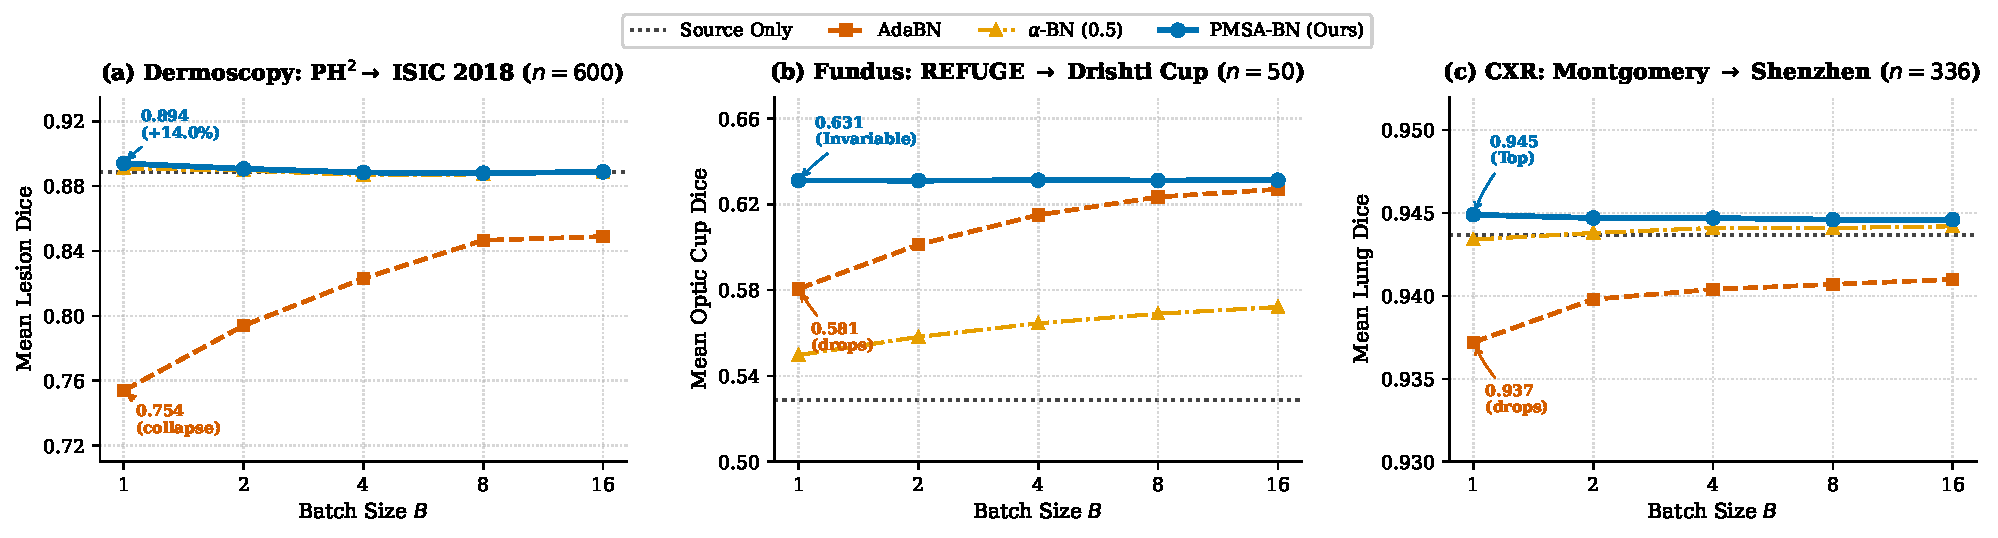
\includegraphics[width=0.68\linewidth]{fig1_batch_size.pdf}
\caption{Dice versus test batch size ($1$--$16$) for AdaBN and PMSA-BN. AdaBN depends on batch statistics and degrades at small batches, whereas PMSA-BN is essentially flat and already at its best at $B=1$.}
\label{fig:batch_size}
\end{figure}

\noindent Representative ablation (PH$^2\to$ISIC18, seed 42, $B=1$, Dice): Source Only ($0.831$); AdaBN ($0.680$); class-conditional split with \emph{target} proportions ($0.666$, confirming that class separation without prior matching leaves label-proportion shift intact); + prior-matched recombination ($0.788$, $+12.2\%$ recovery); + empirical Bayes shrinkage ($0.840$, $+5.2\%$ from small-sample stability); + per-channel $\alpha_c$ mixing ($0.834$); + second pass ($0.835$). Stratification by lesion area confirms that AdaBN's $B=1$ collapse is concentrated on small lesions (Q1 $<7.5\%$ area: AdaBN collapses to $0.242$ Dice, whereas PMSA-BN preserves $0.775$). Variants with a border-aware gate or an $\alpha$-BN first pass changed Dice by $<0.002$; an AdaBN first pass was lower by $0.007$. Replacing pseudo-masks with ground-truth masks (Oracle) gave $0.840$ ($+0.006$), indicating limited headroom from pseudo-mask refinement. As shown in Figure~\ref{fig:batch_size}, AdaBN requires large batches ($B=16$) to partially recover from its $B=1$ collapse ($0.680 \to 0.807$), whereas PMSA-BN remains essentially flat across all batch sizes ($0.834$ at $B=1$, $0.832$ at $B=16$).

%=====================================================================
\section{Scope and limitations}
\begin{itemize}
\item Requires a backbone with BatchNorm. nnU-Net uses InstanceNorm by default, so the method does not apply to it directly.
\item Requires one labelled pass over the source data after training (Phase~0). No source images are needed at test time.
\item Relies on pass-1 pseudo-masks; under very severe shift these may be poor.
\item Gains over Source Only are modest when the source model is already strong; the larger benefit is robustness (avoiding the AdaBN collapse) without choosing a mixing weight per target.
\item Derm7pt uses automatically generated reference contours and should be read as a supplementary check.
\item Novelty must be confirmed against prior work on class-conditional BN, label-shift-aware normalization and statistic-mixing TTA (e.g.\ $\alpha$-BN, DUA, SITA, VPTTA) before submission.
\end{itemize}

\end{document}
